\section{Motivation}\label{sec:2:motivation}

The shift from fine-granular predictive process monitoring including next activity, remaining time, and outcome prediction, to model-based prediction, allows to obtain new insights into the global development of the process.
Consider the example in Figure \ref{fig:dfg_example_intro} where the road fine traffic management event log\footnote{\url{https://doi.org/10.4121/uuid:270fd440-1057-4fb9-89a9-b699b47990f5}} is partitioned into 100 intervals in which an equal number of DF relations occur.
\begin{figure}
    \centering
    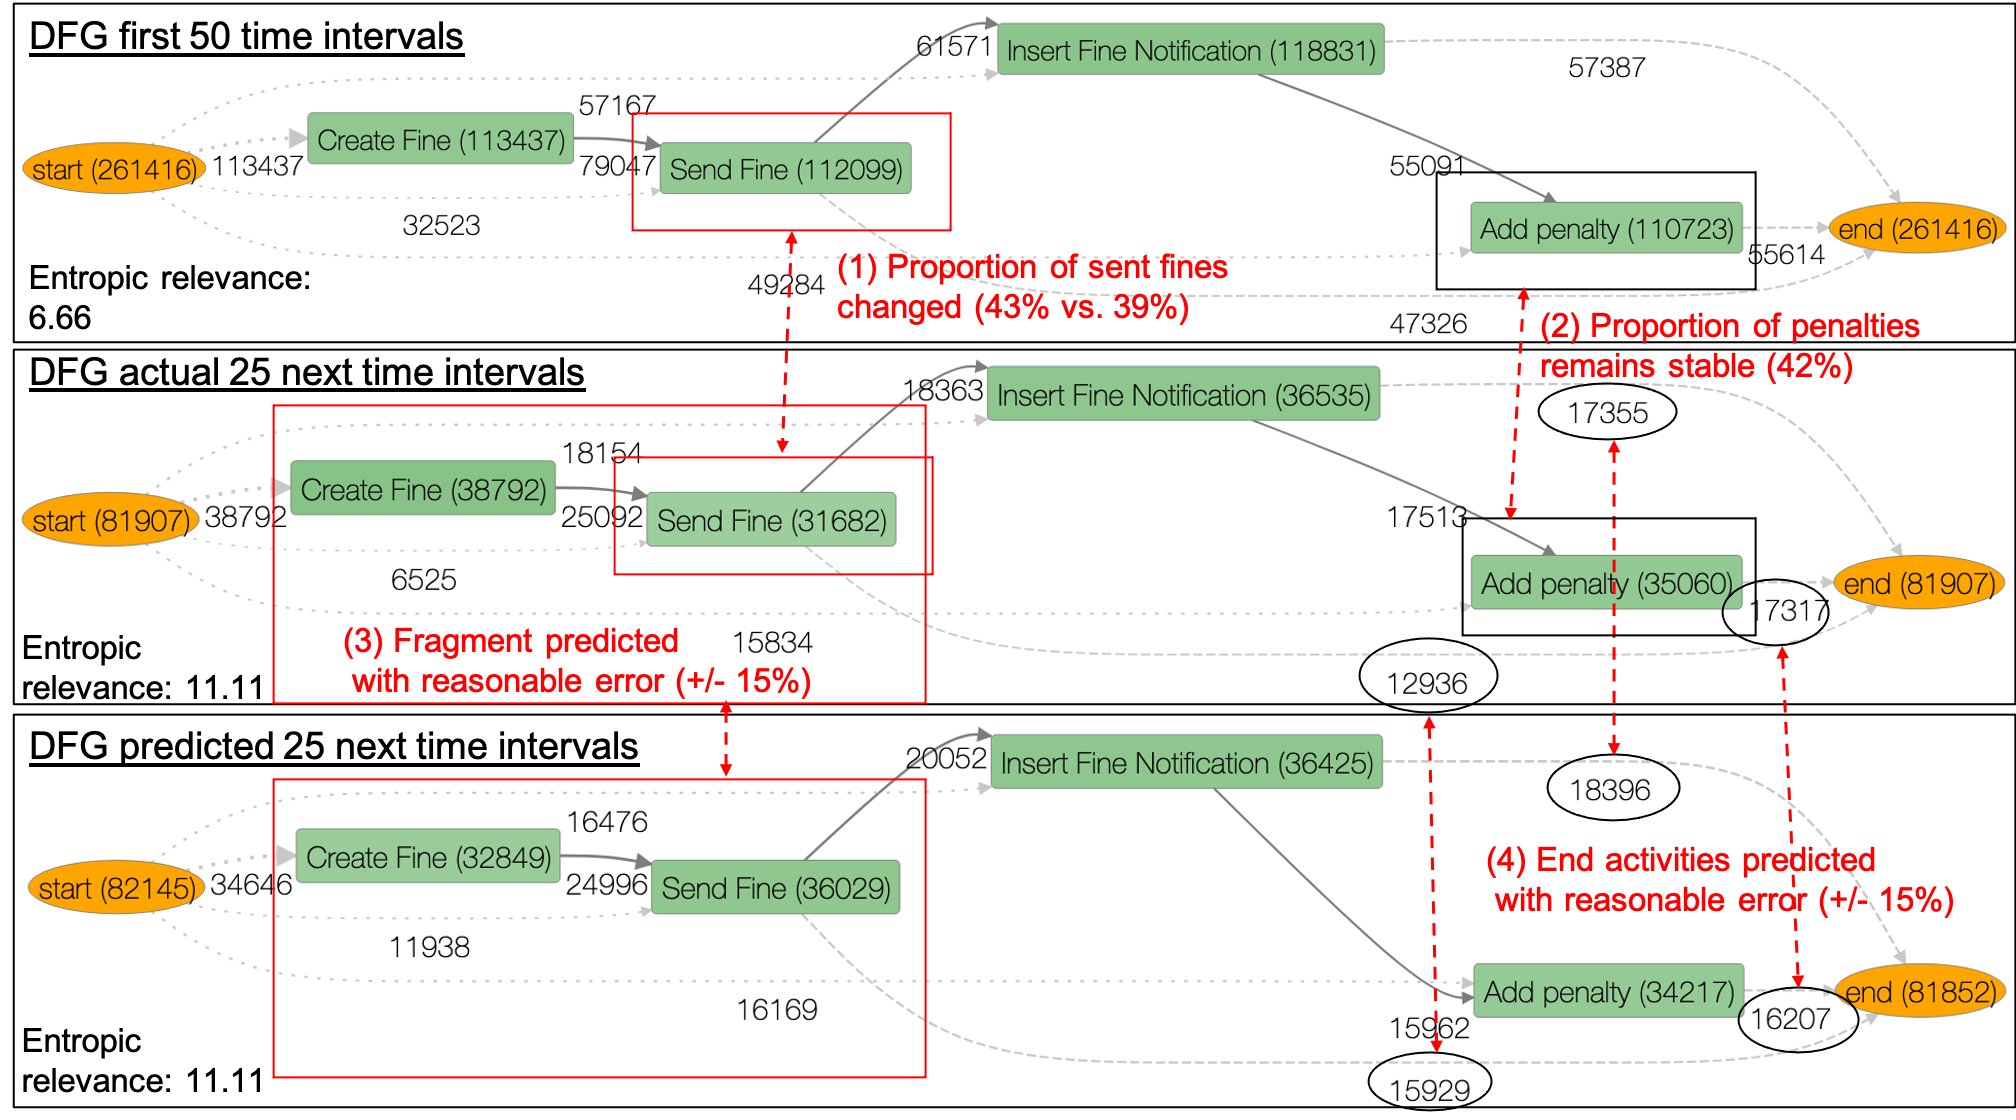
\includegraphics[width=\textwidth]{img/MotExample.png}
    \caption{Directly-follows graphs of the 45 first intervals of the event log, as well as a forecasted and actual DFG of the 25 next intervals.}
    \label{fig:dfg_example_intro}
\end{figure}
The DFs in the first 50 intervals are used to predict the next 25 intervals.
The DFGs show how process model forecasting and change exploration can provide multiple unique insights at a glance:
\begin{enumerate}
    \item Compared to the initial 50 intervals the proportion of fines sent decreases in the later intervals;
    \item The number of penalties added remains comparable between the first 50 and next 25 time intervals;
    \item The number of occurrences and arc weights between \emph{Create Fine} and \emph{Send Fine} are predicted with reasonable error (+\-15\%)
    \item The arc weights of the ending activities are predicted with reasonable error (+\-15\%)
\end{enumerate}
These provide insight both in terms of the past en present model ((1)-(2)) and the quality of forecasts between the actual and forecasted model ((3)-(4)).
Being able to construct such forecasts allows stakeholders to make estimates regarding how the overall fine system will evolve and allows to answer questions such as `How many more fines will be received?', `Will the backlog of fines be reduced?', `Will all fines be paid', and `Will the ratio of unpaid fines stay the same?'
This motivating example shows that, where process mining/monitoring focuses on learning the as-is model to reason about a to-be model and suggest potential repairs and improvements, process model forecasting allows to already grasp the future outcomes of the current as-is process, which allows to shortcut potentially wrong outcomes. 

We evaluate the forecasts quantitatively using entropic relevance \cite{DBLP:conf/icpm/PolyvyanyyMG20} to measure the quality of the discovered and forecasted DFGs with respect to the event logs they represent. 
Entropic relevance penalises the discrepancies in the relative frequencies of traces recorded in the log and described by the DFG. Entropic relevance stands for the average number of bits used to encode a log trace using the DFG, with small values being preferable to large ones.
The entropic relevance of the forecasted DFG and the actual future DFG with respect to the test log is the same, suggesting that both DFGs represent the future behaviour similarly well. 
The entropic relevance of the historical DFG derived from the training log with respect to the testing log is X, suggesting that the future behaviour shifts and the historical DFG does not describe the testing log well enough. 
Finally, the DFG that describes all and only traces of the testing log with the relative frequencies as they are observed in the log has the entropic relevance with the testing log of Y, the best possible relevance value for this log. As the difference between 4.64 and Y is small, we conclude that the forecasted DFG approximates the actual future behaviour well and much better than the historical DFG.

In this light, we complement the model-level prediction technique with a visualisation system to enable analysts to understand the forthcoming changes to the processes. The authors of~\cite{DBLP:conf/bpm/PollPRRR18} discuss the opportunities for process forecasting. They describe that the utility of process forecasting is an understanding of the incremental changes or adaptations that happen to the process model into the future. In terms of visualisation principles, we follow the "Visual Information-Seeking Mantra":~\emph{overview first, zoom and filter, then details-on-demand}~\cite{DBLP:conf/vl/Shneiderman96}. 
%(maybe talk about tasks? not requirements)
Thus, we expect the design of our visualisation system to assist in the following tasks:

\begin{requidescr}
	\item[Identify process adaptations:\namedlabel{req:adaptation}] The visualisation system should assist the user in identifying the changes that happen in the process model of the future in respect to the past;
	\item[Allow for interactive exploration:\namedlabel{req:interactive}] The user should be able to follow the visual information-seeking principles, including overview first, filtering, zooming, and details-on-demand.
\end{requidescr} % CUSTOM from CDC, with love :)

Observe that our process model forecasting technique intrinsically puts forwards an entirely new perspective on predictive process monitoring. The prediction horizon is much longer compared to what existing next-activity prediction models can achieve. Moreover, where next-activity and related predictive algorithms have a strong case-level focus, our technique centres on model-level prediction to obtain a full picture of the future development of a process (model). Please note that process model forecasting could partially assume goal-oriented prediction, as the forecast DFG allows to answer multiple oftentimes used goal statements pertaining to the execution of a particular activity, or a precedence relationship of a particular activity pair \cite{DBLP:journals/tkdd/TeinemaaDRM19} at the same time. However, our technique is not intended to ``replace'' existing techniques, but rather puts forward an entirely new perspective.

%Note that the horizon is longer compared with next-step prediction, and that these results would only be obtainable if long next-step predictions were performed.
%Hence, both are complementary by their being used as varying horizons to obtain a full picture of the future development of a process (model).
%Process model forecasting remains complementary with remaining time prediction as well, which could indicate what activities lead to what remaining time.
%The process model forecast can partially assume goal-oriented prediction, as the forecast DFG allows to answer multiple oftentimes used goal statements pertaining to the execution of a particular activity, or a precedence relationship of a particular activity pair \cite{DBLP:journals/tkdd/TeinemaaDRM19} at the same time.
